\section{Introduction of the Physical Problem}
    \begin{frame}[t]
        \frametitle{Particle Types}
        
        \vspace{-0.4cm}

        \begin{minipage}[t]{0.5\textwidth}
            \vspace{0pt}
            \begin{itemize}
                \item Bosonic operators \pause
                \begin{itemize} 
                    \item Commutation relations
                \end{itemize}
            \end{itemize}
        \end{minipage}%
        \onslide
        \hfill
        \begin{minipage}[t]{0.45\textwidth}
            \vspace{0pt}
            \makebox[\textwidth][c]{
                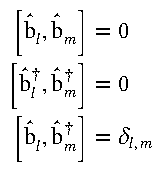
\includegraphics[width=0.5\textwidth]{./main-content/introduction/bosonic-operators.pdf}
            }
        \end{minipage}

        % notes 
        \onslide % on all slides of frame
        \note[item] {
            TODO
        }
    \end{frame}

    \begin{frame}[t]
        \frametitle{Particle Types}
        
        \vspace{-0.4cm}

        \begin{minipage}[t]{0.5\textwidth}
            \vspace{0pt}
            \begin{itemize}
                \item Bosonic operators
                \begin{itemize}
                    \item Commutation relations
                \end{itemize}
                \item Fermionic operators \pause
                \begin{itemize}
                    \item Anti-commutation relations
                \end{itemize}
            \end{itemize}
        \end{minipage}%
        \onslide
        \hfill
        \begin{minipage}[t]{0.45\textwidth}
            \vspace{0pt}
            \makebox[\textwidth][c]{
                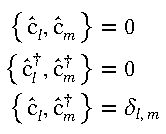
\includegraphics[width=0.5\textwidth]{./main-content/introduction/fermionic-operators.pdf}
            }
        \end{minipage}

        % notes 
        \onslide % on all slides of frame
        \note[item] {
            TODO
        }
    \end{frame}

    \begin{frame}[t]
        \frametitle{Particle Types}
        
        \vspace{-0.4cm}

        \begin{minipage}[t]{0.5\textwidth}
            \vspace{0pt}
            \begin{itemize}
                \item Bosonic operators
                \begin{itemize}
                    \item Commutation relations
                \end{itemize}
                \item Fermionic operators
                \begin{itemize}
                    \item Anti-commutation relations
                \end{itemize}
                \item Hard-core bosonic operators \pause
                \begin{itemize}
                    \item Commutation relations \pause
                    \item Occupation number limited to 0 and 1  \pause
                    \item Number operator is idempotent
                \end{itemize}
            \end{itemize}
        \end{minipage}%
        \onslide
        \hfill
        \begin{minipage}[t]{0.45\textwidth}
            \vspace{0pt}
            \makebox[\textwidth][c]{
                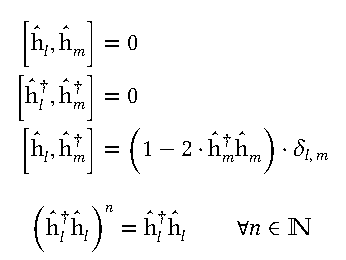
\includegraphics[width=0.85\textwidth]{./main-content/introduction/hard-core-bosonic-operators.pdf}
            }
        \end{minipage}

        % notes 
        \onslide % on all slides of frame
        \note[item] {
            TODO
        }
    \end{frame}

    \begin{frame}[t]
        \frametitle{Particle Types}
        
        \vspace{-0.4cm}

        \begin{minipage}[t]{0.5\textwidth}
            \vspace{0pt}
            \begin{itemize}
                \item Bosonic operators
                \begin{itemize}
                    \item Commutation relations
                \end{itemize}
                \item Fermionic operators
                \begin{itemize}
                    \item Anti-commutation relations
                \end{itemize}
                \item Hard-core bosonic operators
                \begin{itemize}
                    \item Commutation relations
                    \item Occupation number limited to 0 and 1
                    \item Number operator is idempotent
                \end{itemize}
                \item Spins (Pauli operators/matrices)\pause
                \begin{itemize}
                    \item Particles from different sites commute
                    \item Different spin directions on the same site anti-commute
                    \item They obey angular momentum commutation relations
                \end{itemize}
            \end{itemize}
        \end{minipage}%
        \onslide
        \hfill
        \begin{minipage}[t]{0.45\textwidth}
            \vspace{-1.0cm}
            \makebox[\textwidth][c]{
                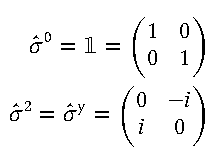
\includegraphics[width=0.55\textwidth,page=1]{./main-content/introduction/spin-operators.pdf}
            }%
            \vspace{-0.3cm}
            \makebox[\textwidth][c]{
                \includegraphics[width=0.55\textwidth,page=2]{./main-content/introduction/spin-operators.pdf}
            }%
            \vspace{-0.1cm}
            \pause[2]
            \makebox[\textwidth][c]{
                \includegraphics[width=0.85\textwidth,page=3]{./main-content/introduction/spin-operators.pdf}
            }
        \end{minipage}

        % notes 
        \onslide % on all slides of frame
        \note[item] {
            TODO
        }
    \end{frame}

    \begin{frame}[t]
        \frametitle{Particle Types - Mappings}
        
        \vspace{-0.4cm}

        \begin{minipage}[t]{0.5\textwidth}
            \vspace{0pt}
            \begin{itemize}
                \item Properties of Pauli matrices \pause
                \begin{itemize}
                    \item Base of the complex 2x2 matrices \pause
                    \item Can be directly mapped to hard-core bosons
                \end{itemize}
            \end{itemize}
        \end{minipage}%
        \onslide
        \hfill
        \begin{minipage}[t]{0.45\textwidth}
            \vspace{0.0cm}
            \pause[3]
            \makebox[\textwidth][c]{
                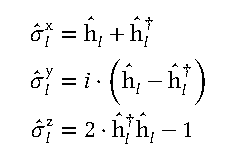
\includegraphics[width=0.6\textwidth,page=1]{./main-content/introduction/transformation.pdf}
            }%
            \vspace{0.1cm}
            \makebox[\textwidth][c]{
                \includegraphics[width=0.95\textwidth,page=2]{./main-content/introduction/transformation.pdf}
            }
        \end{minipage}

        % notes 
        \onslide % on all slides of frame
        \note[item] {
            TODO
        }
    \end{frame}